\chapter{HASIL DAN PENGUJIAN}
\vspace{1ex}

\section*{}
Pada bab ini dipaparkan hasil pengujian serta analisa dari de-
sain sistem dan implementasi .Pengujian dilakukan guna mengetahui tingkat kesalahan dan menarik kesimpulan dari sistem yang telah dibuat.

Pada pengujian ini digunakan \textit{Smartphone Android} dengan spesifikasi hardware seperti pada tabel \ref{tabel:4.0}.
\begin{table}[h!]
		\caption{Spesifikasi \textit{Smartphone} yang Digunakan}
	\begin{tabular}{|l|l|}
		\hline
		\textbf{CPU} & \begin{tabular}[c]{@{}l@{}}Octa-core (4x1.8 GHz Kryo 260 Gold \\ \& 4x1.6 GHz Kryo 260 Silver)\end{tabular} \\ \hline
		\textbf{Internal}       & \begin{tabular}[c]{@{}l@{}}32GB 3GB RAM\end{tabular}  \\ \hline
		\textbf{Chipset}          & Qualcomm SDM636 Snapdragon 636 (14 nm)             \\ \hline
		\textbf{OS}     & Android 8.1 (Oreo), upgradable to Android 9.0 (Pie) \\ \hline
		\textbf{GPU} & Adreno 509         \\ \hline
		\textbf{Bluetooth} & 5.0, A2DP, LE         \\ \hline
	\end{tabular}
	\vspace{1ex}
	\caption{Spesifikasi \textit{Smartphone} yang Digunakan}
	\label{tabel:4.0}
\end{table}




\section{Pengujian Rekaman Data Selama 15 Menit}
\vspace{1ex}
Pengujian ini dilakukan untuk menentukan baudrate bluetooth HC-05 yang akan digunakan dan delay yang diprogram pada arduino. Pada pengujian ini dilakukan dengan cara melakukan rekaman data dengan target durasi rekaman adalah 15 menit. Untuk menentukan delay dan baudrate yang akan digunakan maka pada pengujian ini dilakukan percobaan dengan delay dan baudrate yang berbeda-beda. Untuk delay sendiri memiliki 3 percobaan yaitu delay 1 ms, delay 5 ms, dan delay 10 ms. Sedangkan baudrate yang digunakan untuk percobaan terdapat 4 tahap yaitu 9600, 38400, 57600, dan 115200. Berikut ini merupakan tabel hasil pengujian rekaman data selama 15 (Tabel \ref{tabel:4.0.0})
\begin{table}[H]
	\caption{Tabel hasil percobaan rekaman data dengan target 15 menit}
	\begin{tabular}{|c|c|c|c|c|}
		\hline
		\multicolumn{1}{|c|}{{\color[HTML]{000000} \textbf{Delay}}} & \multicolumn{1}{|c|}{\textbf{Baudrate}} &
		\multicolumn{1}{|c|}{ \textbf{\textit{Force}}} &
		\multicolumn{1}{|c|}{\textbf{Durasi}} &
		\multicolumn{1}{|c|}{\textbf{Sampling}}  \\
		(ms) &  \textbf{HC-05}  & \textbf{\textit{close}}  & \textbf{dicapai} & \textbf{rate}  \\
		&  &  &   & (sampel/detik)  \\ \hline
		
		10 & 9600 & tidak & 15 menit & 50  \\ \hline
		5 & 9600 & ya & 2 menit & 68  \\
		& & & 58.20 detik & \\ \hline
		1 & 9600 & ya & 4 menit & 90  \\ & & & 22.98 detik & \\\hline
		10 & 38400 & ya & 3 menit & 72  \\ & & & 23.65 detik & \\\hline
		5 & 38400 & ya & 1 menit & 114  \\ & & & 52.64 detik & \\ \hline
		1 & 38400 & ya & 2 menit & 216  \\ & & & 14.68 detik & \\ \hline
		10 & 57600 & ya & 2 menit & 112  \\ & & & 05.98 detik & \\ \hline
		5 & 57600 & ya & 2 menit & 125  \\ & & & 51.81 detik & \\ \hline
		1 & 57600 & ya & 2 menit & 270  \\ & & & 23.52 detik & \\ \hline
		10 & 115200 & ya & 3 menit & 117  \\ & & & 52.15 detik & \\ \hline
		5 & 115200 & ya & 1 menit & 139  \\ & & & 42.05 detik & \\ \hline
		1 & 115200 & ya & 1 menit & 327  \\ & & & 36.90 detik & \\ \hline
		
	\end{tabular}
	\vspace{1ex}
	
	\label{tabel:4.0.0}
\end{table}

Dapat dilihat pada tabel diatas memiliki 5 kolom yaitu Delay, Baudrate HC-05, Force close, Durasi dicapai, dan Frekuensi sampling. Delay merupakan durasi jeda waktu yang digunakan pada loop arduino. Baudrate HC-05 merupakan kecepatan pengiriman data oleh modul bluetooth HC-05. Force close merupakan kejadian dimana aplikasi menutup dengan sendirinya. Durasi dicapai merupakan lama waktu rekaman yang telah didapat sampai dengan aplikasi force close. Frekuensi sampling merupakan jumlah data atau sampel yang didapat selama satu detik.

Pada percobaan pertama dilakukan dengan menggunakan delay 10 ms, baudrate HC-05 sebesar 9600, dan frekuensing sampling sebesar 50 data/detik. Pada percobaan pertama berjalan lancar hingga aplikasi dapat merekam data selama 15 menit. Percobaan kedua dilakukan dengan mengubah delay arduino menjadi 5 ms, frekuensi sampling yang didapat adalah 68 data/detik, pada percobaan ini aplikasi tertutup dengan sendirinya (\textit{force close}) setelah merekam selama 2 menit 58.20 detik. Percobaan ketiga dilakukan menggunakan delay 1 ms, dengan baudrate tetap sebesar 9600, frekuensi sampling yang diperoleh sebesar 90 data/detik, pada percobaan ketiga aplikasi mengalami \textit{force close} setelah merekam selama 4 menit 22.98 detik. Percobaan keempat menggunakan delay 10 ms, dengan baudrate HC-05 diperbesar menjadi 38400, frekuensi sampling pada percobaan ini sebesar 72 data/detik, pada percobaan keempat ini aplikasi juga mengalami \textit{force close} setelah merekam selama 3 menit 23.65 detik. Percobaan kelima menggunakan delay sebesar 5 ms, dengan baudrate 38400, frekuensi sampling yang diperoleh
sebesar 114 data/detik, dan seperti sebelumnya aplikasi mengalami \textit{force close} setelah merekam selama 1 menit 52.64 detik. Percobaan keenam dilakukan menggunakan delay sebesar 1 ms, dengan baudrate yang sama yaitu 38400, frekuensi sampling yang diperoleh sebesar 216 data/detik, aplikasi mengalami \textit{force close} setelah merekam selama 2 menit 14.68 detik. Pada percobaan ketujuh aplikasi juga mengalami \textit{force close}, durasi yang dicapai selama 2 menit 05.98 detik, percobaan ini menggunakan delay arduino sebesar 10 ms, dengan baudrate yang diperbesar menjadi 57600, dan frekuensi sampling yang diperoleh sebesar 112 data/detik. Percobaan kedelapan dilakukan menggunakan delay arduino sebesar 5 ms, dengan baudrate sebesar 57600, diperoleh frekuensi sampling sebesar 125 data/detik, aplikasi mengalami \textit{force close} setelah merekam selama 2 menit 51.81 detik. Percobaan kesembilan dilakukan dengan menggunakan delay arduino sebesar 1 ms, dengan baudrate sebesar 57600, diperoleh frekuensi sampling sebesar 270, aplikasi mengalami \textit{force close} setelah merekam selama 2 menit 23.52 detik. Percobaan kesepuluh dilakukan dengan menggunakan delay arduino sebesar 10 ms, dengan baudrate diperbesar menjadi 115200, frekuensi sampling yang diperoleh sebesar 117 data/detik, aplikasi mengalami \textit{force close} setelah merekam selama 3 menit 52.15 detik. Percobaan kesebelas dilakukan menggunakan delay arduino sebesar 5 ms, dengan baudrate sebesar 115200, frekuensi sampling yang diperoleh sebesar 139 data/detik. Percobaan kedua belas yang merupakan percobaan terakhir menggunakan delay arduino sebesar 1 ms, dengan baudrate sebesar 115200, frekuensi sampling yang diperoleh sebesar 327 data/detik. Pada percobaan terakhir ini aplikasi juga mengalami \textit{force close}, \textit{force close} tersebut terjadi setelah merekam selama 1 menit 36.90 detik. 

Berdasarkan tabel \ref{tabel:4.0.0} dapat dilihat pada kolom force dimana hampir pada semua percobaan yang telah dilakukan mengalami force close pada aplikasi. Apabila dilihat pada kolom durasi dicapai, durasi waktu yang didapat saat aplikasi force close tidak pasti, tetapi sebagian besar aplikasi mengalami force close pada menit ke-2. Sedangkan apabila kolom Force close dihubungkan kolom Frekuensi sampling
maka aplikasi hanya dapat berjalan dengan baik hingga menit ke-15 dengan menggunakan fruekuensi sampling 50 sampel/detik, untuk frekuensi selain 50 sampel/detik tersebut aplikasi mengalami force close. Berdasarkan analisa maka dapat  semakin besar frekuensi sampling yang digunakan maka semakin besar kemungkinan force close pada aplikasi.


\section{Pengujian Persentase Data Hilang}
\vspace{1ex}
Pada bagian ini, pengujian dilakukan dengan cara merekam data ECG yang dikirimkan oleh arduino. Pada pengujian ini menggunakan \textit{baudrate} sebesar 9600. Pengujian ini dilakukan untuk mengetahui seberapa banyak data yang hilang dengan cara membandingkan data yang dikirim oleh mikrokontroler arduino dengan data yang diterima oleh aplikasi. Berikut adalah tabel yang merupakan hasil percobaan selama 1 menit (Tabel \ref{tabel:4.1}).
\begin{table}[H]
	\caption{Tabel hasil percobaan persentase data hilang}
	\begin{tabular}{|c|c|c|c|c|c|}
		\hline
		\multicolumn{1}{|c|}{{\color[HTML]{000000} \textbf{Delay}}} & \multicolumn{1}{|c|}{\textbf{Jumlah}} &
		\multicolumn{1}{|c|}{ \textbf{Jumlah}} &
		\multicolumn{1}{|c|}{\textbf{Waktu}} &
		\multicolumn{1}{|c|}{\textbf{Frekuensi}} &
		\multicolumn{1}{|c|}{\textbf{Data}} \\
		(ms) & \textbf{Data} & \textbf{Data} & \textbf{uji} & \textbf{samplin}g & \textbf{hilang } \\
		& \textbf{dikirim} & \textbf{diterima} & (s)  & (sampel/detik) & (\%) \\ \hline
		100 & 543 & 542 & 60 & 9 & 0.19 \\ \hline 
		10 & 3107 & 3098 & 60 & 51 & 0.29 \\ \hline
		5 & 4168 & 4143 & 60 & 69 & 0.6 \\ \hline
		1 & 5748 & 5727 & 60 & 95 & 0.37 \\ \hline
			
	\end{tabular}
	\vspace{1ex}
	
	\label{tabel:4.1}
\end{table}
Tabel \ref{tabel:4.1} merupakan tabel yang memiliki 6 kolom yaitu Delay, Jumlah Data dikirim, Jumlah Data diterima, Waktu uji, Frekuensi sampling, Data hilang. Delay merupakan durasi jeda waktu pada loop arduino. Jumlah Data dikirim merupakan banyak data yang dikirim oleh arduino menuju aplikasi. Jumlah Data diterima merupakan banyak data yang telah sampai di aplikasi. Waktu uji merupakan durasi melakukan pengujian. Frekuensi sampling merupakan banyak data yang diterima aplikasi pada setiap detik. Data hilang merupakan jumlah data yang tidak berhasil sampai pada aplikasi.

Pada pengujian ini, percobaan pertama dilakukan dengan menggunakan delay arduino sebesar 100 ms, jumlah data yang dapat dikirim sebanyak 543, jumlah data yang telah diterima pada aplikasi sebanyak 542, dengan frekuensi sampling sebesar 9 data/detik, dan diperoleh dengan cara perhitungan matematis data yang hilang sebesar 0.19\%. Percobaan kedua dilakukan dengan menggunakan delay arduino sebesar 10 ms, jumlah data yang dapat dikirim sebanyak 3107, jumlah data yang telah diterima pada aplikasi sebanyak 3098, dengan frekuensi sampling sebesar 51 data/detik, dan diperoleh dengan cara perhitungan matematis data yang hilang sebesar 0.29\%. Percobaan ketiga dilakukan dengan menggunakan delay arduino sebesar 5 ms, jumlah data yang dapat dikirim sebanyak 4168, jumlah data yang telah diterima pada aplikasi sebanyak 4143, dengan frekuensi sampling sebesar 69 data/detik, dan diperoleh dengan cara perhitungan matematis data yang hilang sebesar 0.6\%. Percobaan kedua dilakukan dengan menggunakan delay arduino sebesar 1 ms, jumlah data yang dapat dikirim sebanyak 5748, jumlah data yang telah diterima pada aplikasi sebanyak 5727, dengan frekuensi sampling sebesar 95 data/detik, dan diperoleh dengan cara perhitungan matematis data yang hilang sebesar 0.37\%

Pada tabel \ref{tabel:4.1} terdapat kolom frekuensi sampling yang mana merupakan jumlah sample yang berhasil diterima oleh aplikasi dalam 1 detik. Perhitungan frekuensi sampling dengan cara perbandingan antara jumlah data diterima dengan waktu uji. Selain itu juga terdapat kolom data hilang dimana merupakan persentase jumlah data yang tidak berhasil
diterima oleh aplikasi. Perhitungan persentase data hilang adalah dengan cara membandingkan selisih jumlah data dikirim dengan jumlah data diterima dengan jumlah data dikirim kemudian dikalikan dengan 100 \%.

\vspace{1ex}

\section{Pengujian Waktu Pengiriman Data Menuju Database}
\vspace{1ex}
Pengujian ini dilakukan untuk mengetahui seberapa lama waktu yang dibutuhkan untuk mengupload data menuju database. Pengujian dilakukan dengan cara merekam data ECG secara bertahap untuk diupload yaitu dari 1 menit sampai 15 menit. Pada pengujian ini baudrate modul HC-05 yang digunakan adalah 9600 dan delay yang digunakan pada arduino sebesar 10 ms serta data diupload menuju server online. Dari masing-masing tahap rekaman tersebut akan dibandingkan berapa waktu yang dibutuhkan untuk upload data. Berikut merupakan tabel hasil pengujian durasi upload data (Tabel \ref{tabel:4.2}).
\begin{table}[H]
	\caption{Tabel hasil percobaan durasi upload}
	\begin{tabular}{|c|c|c|c|}
		\hline
		\multicolumn{1}{|c|}{{\color[HTML]{000000} \textbf{Durasi}}} & \multicolumn{1}{|c|}{\textbf{Jumlah}} &
		\multicolumn{1}{|c|}{ \textbf{Jumlah}} &
		\multicolumn{1}{|c|}{\textbf{Durasi}}  \\
		\textbf{rekaman} & \textbf{Data} & \textbf{Data} & \textbf{upload} \\
		& \textbf{dikirim} & \textbf{diterima} &    \\ \hline
		1 menit& 3004 & 2992 & 3.60 detik  \\ \hline 
		2 menit& 5876 & 5860 & 6.16 detik   \\ \hline
		3 menit& 8927 & 8911 & 12.83 detik   \\ \hline
		4 menit& 11814 & 11753 & 16.30 detik   \\ \hline
		5 menit& 14699 & 14659 & 17.06 detik   \\ \hline
		6 menit& 17651 & 17583 & 22.61 detik  \\ \hline
		7 menit& 20510 & 20465 & 33.96 detik   \\ \hline
		8 menit& 23382 & 23330 & 19.98 detik   \\ \hline
		9 menit& 26330 & 26279 & 1 menit    \\ 
		& & & 31.64 detik  \\ \hline
		10 menit& 29007 & 28924 & 34.72 detik   \\ \hline
		11 menit & 31848 & 31784 & 22.69 detik   \\ \hline
		12 menit& 33339 & 33260 & 19.25 detik   \\ \hline
		13 menit& 35567 & 35513 & 23.07 detik   \\ \hline
		14 menit& 38312 & 38244 & 28.66 detik   \\ \hline
		15 menit& 41073 & 40973 & 27.01 detik   \\ \hline
	\end{tabular}
	\vspace{1ex}
	
	\label{tabel:4.2}
\end{table}

Dapat dilihat dari tabel diatas memiliki 4 kolom yaitu Durasi rekaman, Jumlah Data dikirim, Jumlah Data diterima, dan Durasi upload. Durasi rekaman merupakan jangka waktu yang dilakukan saat merekam data. Jumlah Data dikirim merupakan jumlah data yang dikirim melalui modul bluetooth HC-05 dari Arduino menuju aplikasi. Jumlah Data diterima merupakan jumlah data yang dapat disampaikan oleh modul bluetooth HC-05 dari Arduino. Dan yang terakhir adalah Durasi upload yang mana merupakan jangka waktu yang diperlukan untuk mengupload data dari aplikasi menuju database.

Pada percobaan pertama dilakukan rekaman selama 1 menit, jumlah data yang terkirim sebanyak 3004 sampel, sedangkan jumlah data yang diterima aplikasi sebanyak 2992 sampel, dan durasi upload ke database selama 3.60 detik. Percobaan kedua dilakukan rekaman selama 2 menit, jumlah data yang dikirim sebanyak 5876 sampel, sedangkan jumlah data yang diterima aplikasi sebanyak 5860 sampel, dan durasi upload ke database selama 6.16 detik. Percobaan ketiga dilakukan rekaman selama 3 menit, jumlah data yang dikirim sebanyak 8927 sampel, sedangkan jumlah data yang diterima aplikasi sebanyak 8911 sampel, dan durasi upload ke database selama 12.83 detik. Percobaan keempat dilakukan rekaman selama 4 menit, jumlah data yang dikirim sebanyak 11814 sampel, sedangkan jumlah data yang diterima aplikasi sebanyak 11753 sampel, dan durasi upload ke database selama 16.30 detik. Percobaan kelima dilakukan rekaman selama 5 menit, jumlah data yang dikirim sebanyak 14699 sampel, sedangkan jumlah data yang diterima aplikasi sebanyak 14659 sampel, dan durasi upload ke database selama 17.06 detik. Percobaan keenam dilakukan rekaman selama 6 menit, jumlah data yang dikirim sebanyak 17651 sampel, sedangkan jumlah data yang diterima aplikasi sebanyak 17583 sampel, dan durasi upload ke database selama 22.61 detik. Percobaan ketujuh dilakukan rekaman selama 7 menit, jumlah data yang dikirim sebanyak 20510 sampel, sedangkan jumlah data yang diterima aplikasi sebanyak 20465 sampel, dan durasi upload ke database selama 33.96 detik. Percobaan kedelapan dilakukan rekaman selama 8 menit, jumlah data yang dikirim sebanyak 23382 sampel, sedangkan jumlah data yang diterima aplikasi sebanyak 23330 sampel, dan durasi upload ke database selama 19.98 detik. Percobaan kesembilan dilakukan rekaman selama 9 menit, jumlah data yang dikirim sebanyak 26330 sampel, sedangkan jumlah data yang diterima aplikasi sebanyak 26279 sampel, dan durasi upload ke database paling lama dari percobaan lainnya yaitu selama 1 menit 31.64 detik.
Percobaan kesepuluh dilakukan rekaman selama 10 menit, jumlah data yang dikirim sebanyak 29007 sampel, sedangkan jumlah data yang diterima aplikasi sebanyak 28924 sampel, dan durasi upload ke database selama 34.72 detik. Percobaan kesebelas dilakukan rekaman selama 11 menit, jumlah data yang dikirim sebanyak 31848 sampel, sedangkan jumlah data yang diterima aplikasi sebanyak 31784 sampel, dan durasi upload ke database selama 22.69 detik. Percobaan kedua belas dilakukan rekaman selama 12 menit, jumlah data yang dikirim sebanyak 33339 sampel, sedangkan jumlah data yang diterima aplikasi sebanyak 33260 sampel, dan durasi upload ke database selama 19.25 detik. Percobaan ketiga belas dilakukan rekaman selama 13 menit, jumlah data yang dikirim sebanyak 35567 sampel, sedangkan jumlah data yang diterima aplikasi sebanyak 35513 sampel, dan durasi upload ke database selama 23.07 detik. Percobaan keempat belas dilakukan rekaman selama 14 menit, jumlah data yang dikirim sebanyak 38312 sampel, sedangkan jumlah data yang diterima aplikasi sebanyak 38244 sampel, dan durasi upload ke database selama 28.66 detik. Percobaan kelima belas yang merupakan percobaan terakhir dilakukan rekaman selama 15 menit, jumlah data yang dikirim sebanyak 41073 sampel, sedangkan jumlah data yang diterima aplikasi sebanyak 40973 sampel, dan durasi upload ke database selama 27.01 detik.

Berdasarkan tabel \ref{tabel:4.2} dapat dilihat perbandingan durasi upload dari jumlah data yang diperoleh selama 1 menit sampai dengan 15 menit. Dari tabel tersebut dapat dilihat durasi upload yang diperlukan tidak pasti atau juga dapat dikatakan tidak linier apabila dibandingkan dengan durasi rekaman. Hal tersebut karena database ada pada server online maka tergantung jaringan internet yang digunakan. Apabila pada saat upload data memiliki jaringan internet yang bagus maka durasi upload akan berjalan lebih cepat. Sebaliknya apablika pada saat upload data memiliki jaringan internet yang kurang bagus maka proses upload akan berjalan lebih lama.

\section{Pengujian kesesuaian data dari arduino dan data di aplikasi}
\vspace{1ex}
Pengujian ini dilakukan untuk melihat perbedaan data yang dikirim dari arduino dengan data yang telah diproses oleh aplikasi. Pengujian ini dilakukan dengan cara melakukan rekaman data selama 1 menit. Percobaan dilakukan sebanyak 5 kali percobaan, data percobaan kemudian dibandingkan 

Data pada arduino ditampilkan menggunakan serial monitor dan untuk aplikasi ditampilkan pada box putih bagian bawah. Dapat dilihat pada gambar \ref{fig:4.2}. Pada gambar tersebut dapat dilihat serial monitor telah menampilkan data yang dikirim oleh arduino terdapat 3 bagian data yaitu \textbf{sampel:data ECG$\mid$detik$\mid$} tetapi data yang dikirim hanya data \textbf{ECG$\mid$detik$\mid$} sedangkan untuk urutan sampel akan diproses pada aplikasi. Hal tersebut dikarenakan sampel pertama yang dikirim dari arduino belum tentu sampai pada aplkasi, maka aplikasi perlu menentukan sampel yang pertama. 
\begin{figure}[H] \centering
	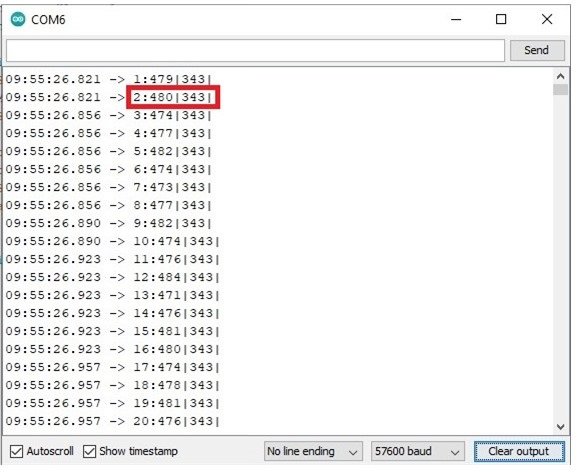
\includegraphics[width=0.7\textwidth]{img/percob/Slide1}

	(a)
	
	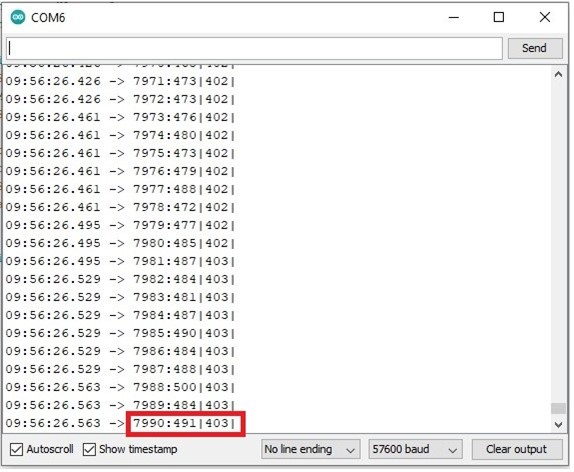
\includegraphics[width=0.7\textwidth]{img/percob/Slide2}
	
	(b)
	
	\caption{Percobaan 1 : (a)Data awal yang dikirim dari arduino, (b)Data akhir yang dikirim arduino.}
	\label{fig:4.2}
\end{figure}
\vspace{1ex}
Dapat dilihat pada Gambar \ref{fig:4.2}, tanda "$\mid$" yang ada pada data tersebut diperlukan untuk melakukan split pada program aplikasi untuk memisahkan data ECG dengan detik. Pada tanda kotak berwarna merah berisi "2:480$\mid$343$\mid$" yang mana angka "2" adalah urutan sampel dari arduino, kemudian angka "480" adalah data sensor, dan "343" merupakan detik. Pada percobaan pertama, data awal yang terkirim oleh arduino adalah 480 pada sampel ke-2 dan data terakhir yang terkirim adalah 491 pada sampel ke-7990. Apabila dihitung maka jumlah sampel yang terkirim adalah 7989 sampel dalam satu menit.
\begin{figure}[H] \centering
	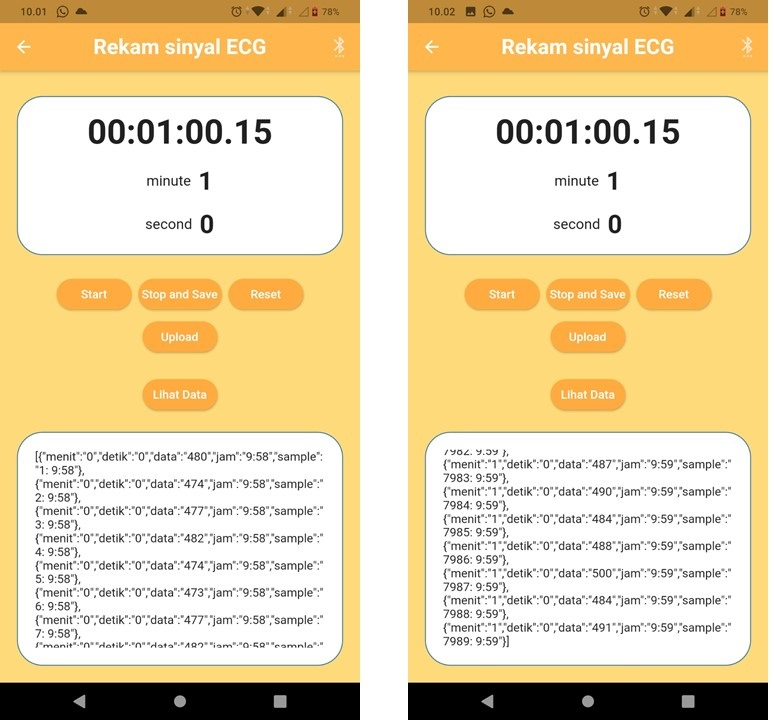
\includegraphics[width=1\textwidth]{img/percob/Slide11}	             
	\caption{Percobaan 1: (kiri) Data awal yang diterima aplikasi, (kanan) Data akhir yang diterima aplikasi.}
	\label{fig:4.2.0}
\end{figure}
\vspace{1ex}
Gambar \ref{fig:4.2.0} merupakan tampilan data yang diterima aplikasi. Dapat dilihat pada gambar tersebut, data yang ada aplikasi adalah menit, detik, data, jam, dan sampel. Menit tersebut didapatkan dari memproses detik yang telah dikirim dari arduino. Detik didapatkan dari data yang dikirim oleh arduino. Data merupakan data ECG yang dikirim oleh arduino. Jam merupakan data penjumlahan antara waktu mulai rekaman dengan detik yang diperoleh dari arduino. Sampel didapat dari proses penomoran data pada aplikasi.  Layar sebelah kiri menunjukkan data pertama yang diterima adalah 480 dan layar sebelah kanan menunjukkan data terakhir yang diterima aplikasi adalah 491. Jumlah data yang diterima oleh aplikasi dapat dilihat pada nomor "sample" yaitu 7989 sampel. Berikutnya adalah gambar percobaan kedua. 
\begin{figure}[H] \centering
	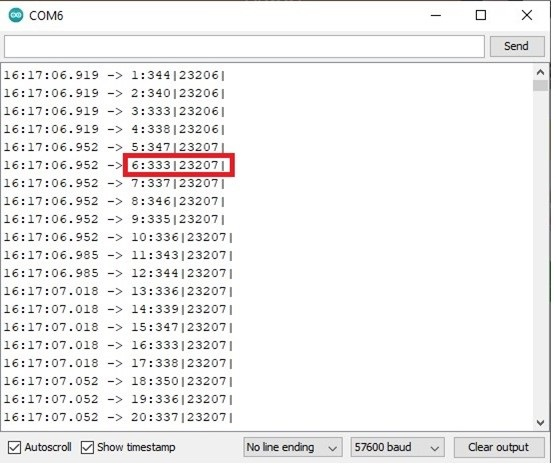
\includegraphics[width=0.7\textwidth]{img/percob/Slide3}
	
	(a)
	
	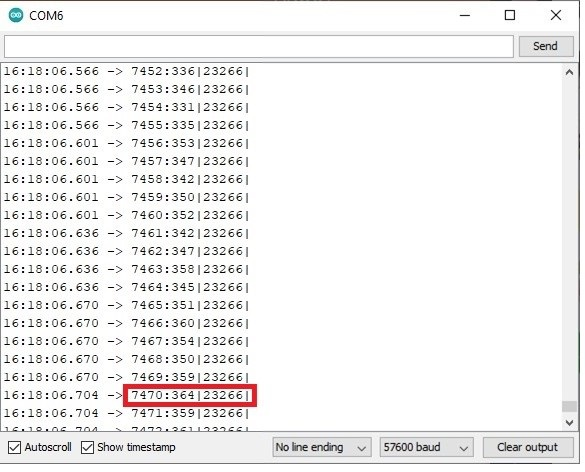
\includegraphics[width=0.7\textwidth]{img/percob/Slide4}
	
	(b)
	
	\caption{Percobaan 2 : (a)Data awal yang dikirim dari arduino, (b)Data akhir yang dikirim arduino.}
	\label{fig:4.2.1}
\end{figure}
\vspace{1ex}
Dapat dilihat pada Gambar \ref{fig:4.2.1}, pada bagian (a) data awal yang terkirim oleh arduino adalah 333 yang merupakan sampel keenam dan pada bagian (b) data terakhir yang terkirim adalah 364 yang merupakan sampel ke-7470. Jumlah data yang dikirim oleh arduino adalah 7465 sampel.

\begin{figure}[H] \centering
	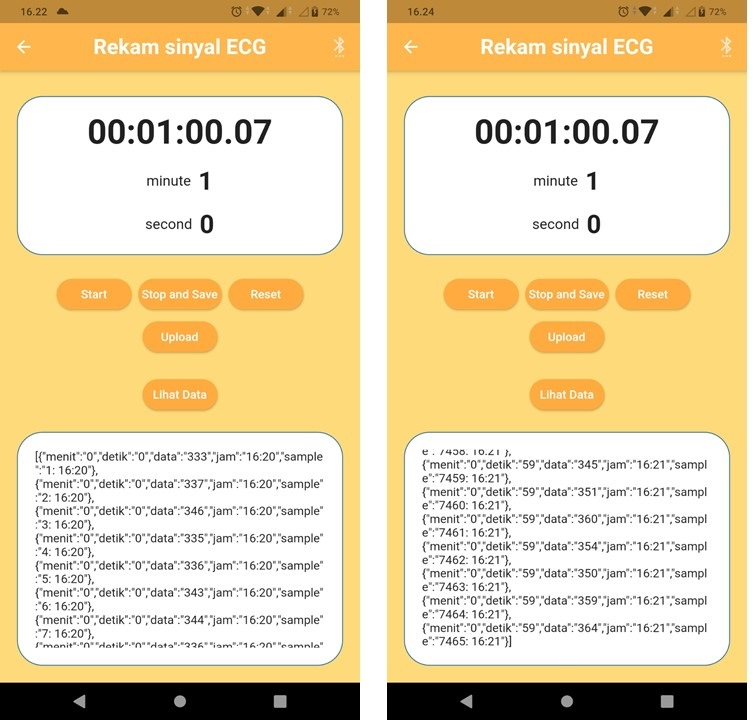
\includegraphics[width=1\textwidth]{img/percob/Slide12}
	\caption{Percobaan 2: (kiri) Data awal yang diterima aplikasi, (kanan) Data akhir yang diterima aplikasi.}
	\label{fig:4.2.2}
\end{figure}
\vspace{1ex}
Gambar \ref{fig:4.2.2} merupakan tampilan data yang diterima aplikasi pada percobaan kedua. Layar sebelah kiri menunjukkan data pertama yang diterima adalah 333 dan layar sebelah kanan menunjukkan data terakhir yang diterima aplikasi adalah 364. Jumlah data yang diterima oleh aplikasi dapat dilihat pada nomor "sample" yaitu 7465 sampel. Berikutnya adalah gambar percobaan ketiga. 

\begin{figure}[H] \centering
	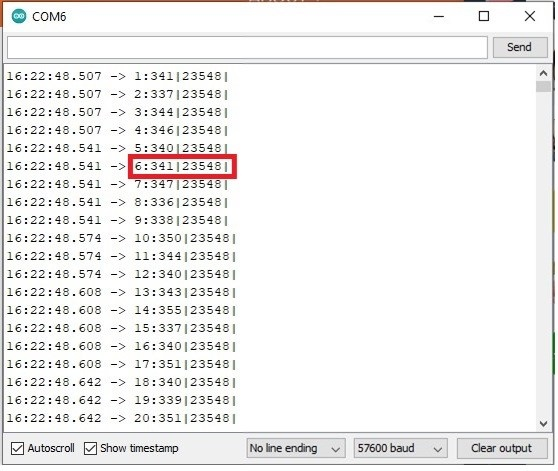
\includegraphics[width=0.7\textwidth]{img/percob/Slide5}
	
	(a)
	
	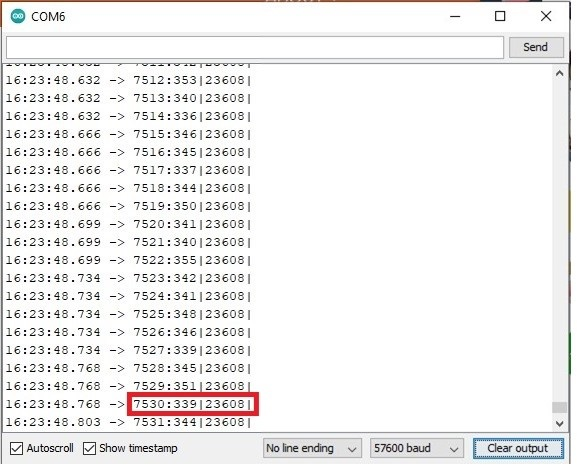
\includegraphics[width=0.7\textwidth]{img/percob/Slide6}
		
	(b)
	
	\caption{Percobaan 3 : (a)Data awal yang dikirim dari arduino, (b)Data akhir yang dikirim arduino.}
	\label{fig:4.2.3}
\end{figure}
\vspace{1ex}
Dapat dilihat pada Gambar \ref{fig:4.2.3}, pada bagian (a) data awal yang terkirim oleh arduino adalah 341 yang merupakan sampel keenam dan pada bagian (b) data terakhir yang terkirim adalah 339 yang merupakan sampel ke-7470. Jumlah data yang dikirim oleh arduino adalah 7525 sampel.

\begin{figure}[!h] \centering
	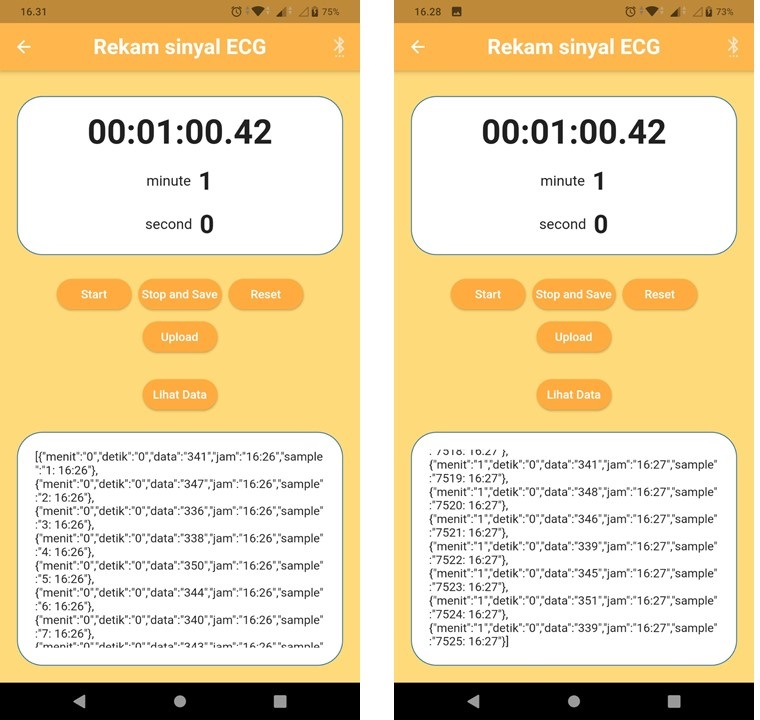
\includegraphics[width=1\textwidth]{img/percob/Slide13}
	\caption{Percobaan 3: (kiri) Data awal yang diterima aplikasi, (kanan) Data akhir yang diterima aplikasi.}
	\label{fig:4.2.4}
\end{figure}
Gambar \ref{fig:4.2.4} merupakan tampilan data yang diterima aplikasi. Layar sebelah kiri menunjukkan data pertama yang diterima adalah 341 dan layar sebelah kanan menunjukkan data terakhir yang diterima aplikasi adalah 339. Jumlah data yang diterima oleh aplikasi dapat dilihat pada nomor "sample" yaitu 7525 sampel. Berikutnya adalah gambar percobaan keempat. 
\begin{figure}[H] \centering
	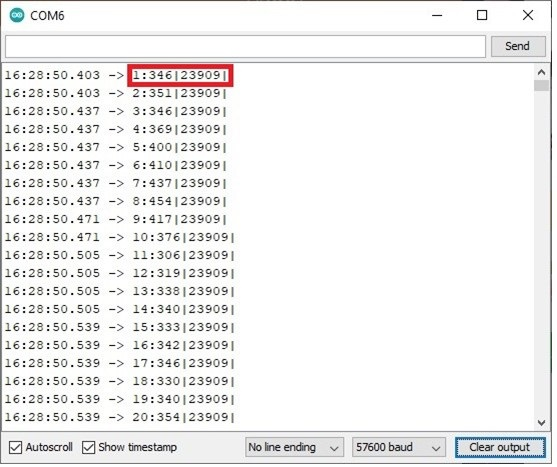
\includegraphics[width=0.7\textwidth]{img/percob/Slide7}
	
	(a)
	
	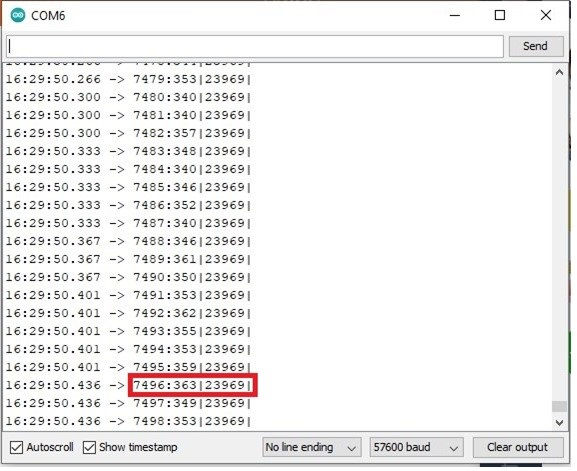
\includegraphics[width=0.7\textwidth]{img/percob/Slide8}
	
	(b)
	
	\caption{Percobaan 4 : (a)Data awal yang dikirim dari arduino, (b)Data akhir yang dikirim arduino.}
	\label{fig:4.2.5}
\end{figure}
\vspace{1ex}
Pada gambar \ref{fig:4.2.5} dapat diketahui bagian (a) data awal yang terkirim adalah 346 yang merupakan sampel pertama pada arduino, kemudian data terakhir ditampilkan pada bagian (b) yaitu 363 merupakan data urutan ke-7496 serta merupakan jumlah data yang berhasil dikirim.


\begin{figure}[H] \centering
	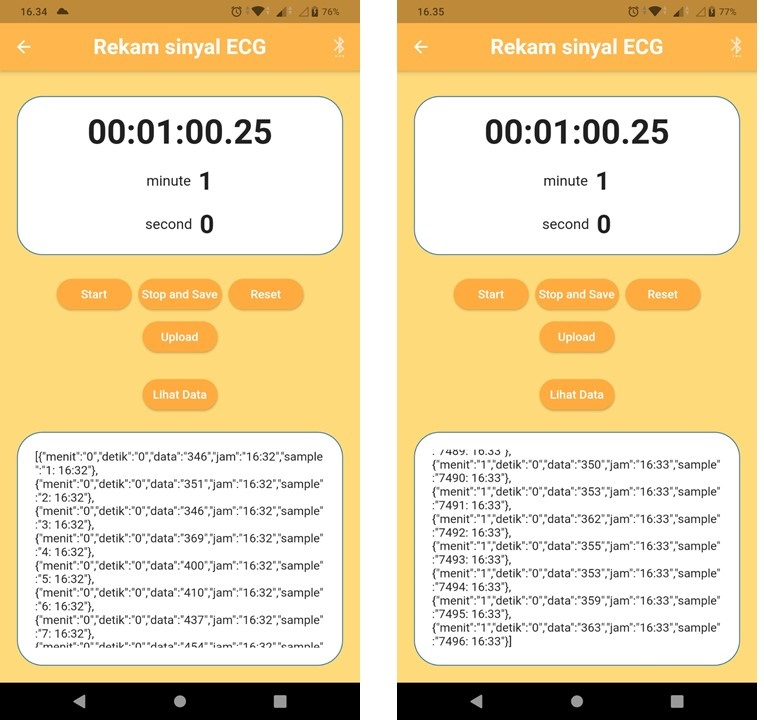
\includegraphics[width=1\textwidth]{img/percob/Slide14}
	\caption{Percobaan 4: (kiri) Data awal yang diterima aplikasi, (kanan) Data akhir yang diterima aplikasi.}
	\label{fig:4.2.6}
\end{figure}
\vspace{1ex}
Pada percobaan keempat seperti yang diperlihatkan Gambar \ref{fig:4.2.6}, pada bagian kiri menunjukkan data awal yang diterima aplikasi yaitu 346 dan pada bagian kanan terdapat data terakhir yang diterima aplikasi yaitu 363. Jumlah data yang diterima aplikasi ditunjukkan pada nomor sampel data terakhir yaitu 7469. Kemudian berikut ini merupakan gambar percobaan terakhir.
\begin{figure}[H] \centering
	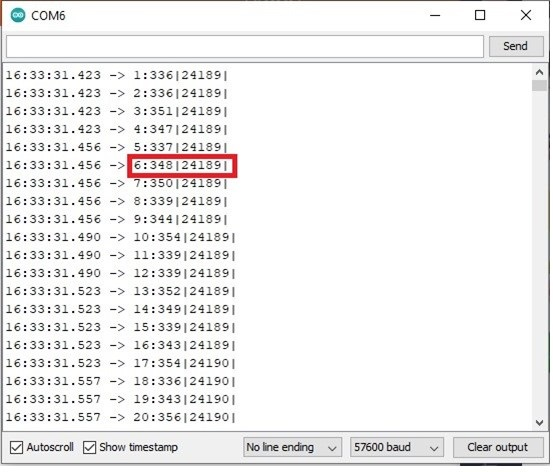
\includegraphics[width=0.7\textwidth]{img/percob/Slide9}
	
	(a)
	
	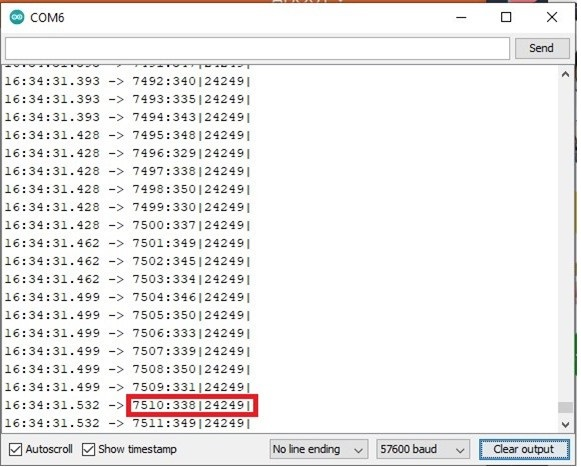
\includegraphics[width=0.7\textwidth]{img/percob/Slide10}
	
	(b)
	
	\caption{Percobaan 5 : (a)Data awal yang dikirim dari arduino, (b)Data akhir yang dikirim arduino.}
	\label{fig:4.2.7}
\end{figure}
\vspace{1ex}
Dapat diketahui dari gambar \ref{fig:4.2.7}, bagian (a) menunjukkan data awal yang terkirim yaitu 348 pada urutan sampel nomor 6, kemudian bagian (b) menunjukkan data terakhir yang terkirim yaitu 338 pada nomor sampel 7510. Apabila diperhitungkan melihat nomor sampel maka jumlah data yang terkirim adalah 7505 sampel.
\begin{figure}[H] \centering
	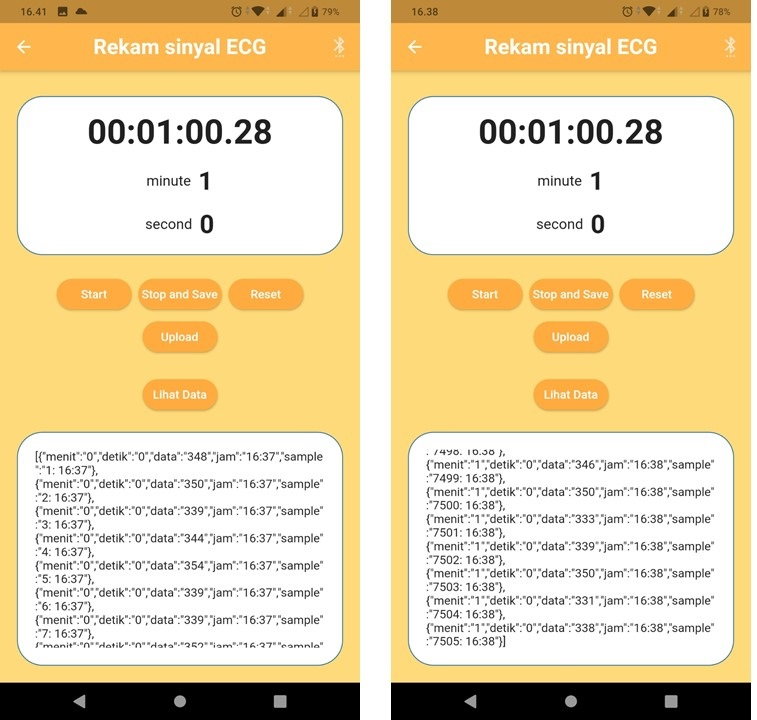
\includegraphics[width=1\textwidth]{img/percob/Slide15}
	\caption{Percobaan 5: (kiri) Data awal yang diterima aplikasi, (kanan) Data akhir yang diterima aplikasi.}
	\label{fig:4.2.8}
\end{figure}
Pada percobaan terakhir didapatkan data seperti yang diperlihatkan Gambar \ref{fig:4.2.8}, pada bagian kiri menunjukkan data awal yang diterima aplikasi yaitu 348 dan pada bagian kanan terdapat data terakhir yang diterima aplikasi yaitu 338. Jumlah data yang diterima aplikasi ditunjukkan pada nomor sampel data terakhir yaitu 7505 sehingga jumlah data yang dikirim arduino sesuai dengan jumlah data yang diterima aplikasi. Untuk lebih jelasnya dapat dilihat pada tabel berikut.

\begin{table}[H]
	\begin{tabular}{|c|c|c|c|c|c|c|}
		\hline
		\multirow{3}{*}{\textbf{Uji ke-}} & \multicolumn{3}{|c|}{\textbf{Arduino}}& \multicolumn{3}{|c|}{\textbf{Aplikasi}}\\
		\cline{2-7} & \textbf{Data} & \textbf{Data} & \textbf{Jumlah}& \textbf{Data}&\textbf{Data}&\textbf{Jumlah}\\
		 & \textbf{awal} & \textbf{akhir} & \textbf{sampel}& \textbf{awal}&\textbf{akhir}&\textbf{sampel}\\
		\hline& & & &&&\\&&&& & & \\& & &&&& \\
		\hline
	\end{tabular}
\end{table}

\section{Pengujian Kesesuian Grafik ECG}
\vspace{1ex}

Pada tahap ini, dilakukan pengujian dengan cara membandingkan grafik ECG yang telah ditampilkan oleh aplikasi android dengan grafik ECG yang ditampilkan oleh serial ploter yang merupakan tools dari Arduino IDE. Berikut adalah hasil grafik ECG yang ditampilkan oleh aplikasi Gambar \ref{fig:4.0}.

\begin{figure}[H] \centering
	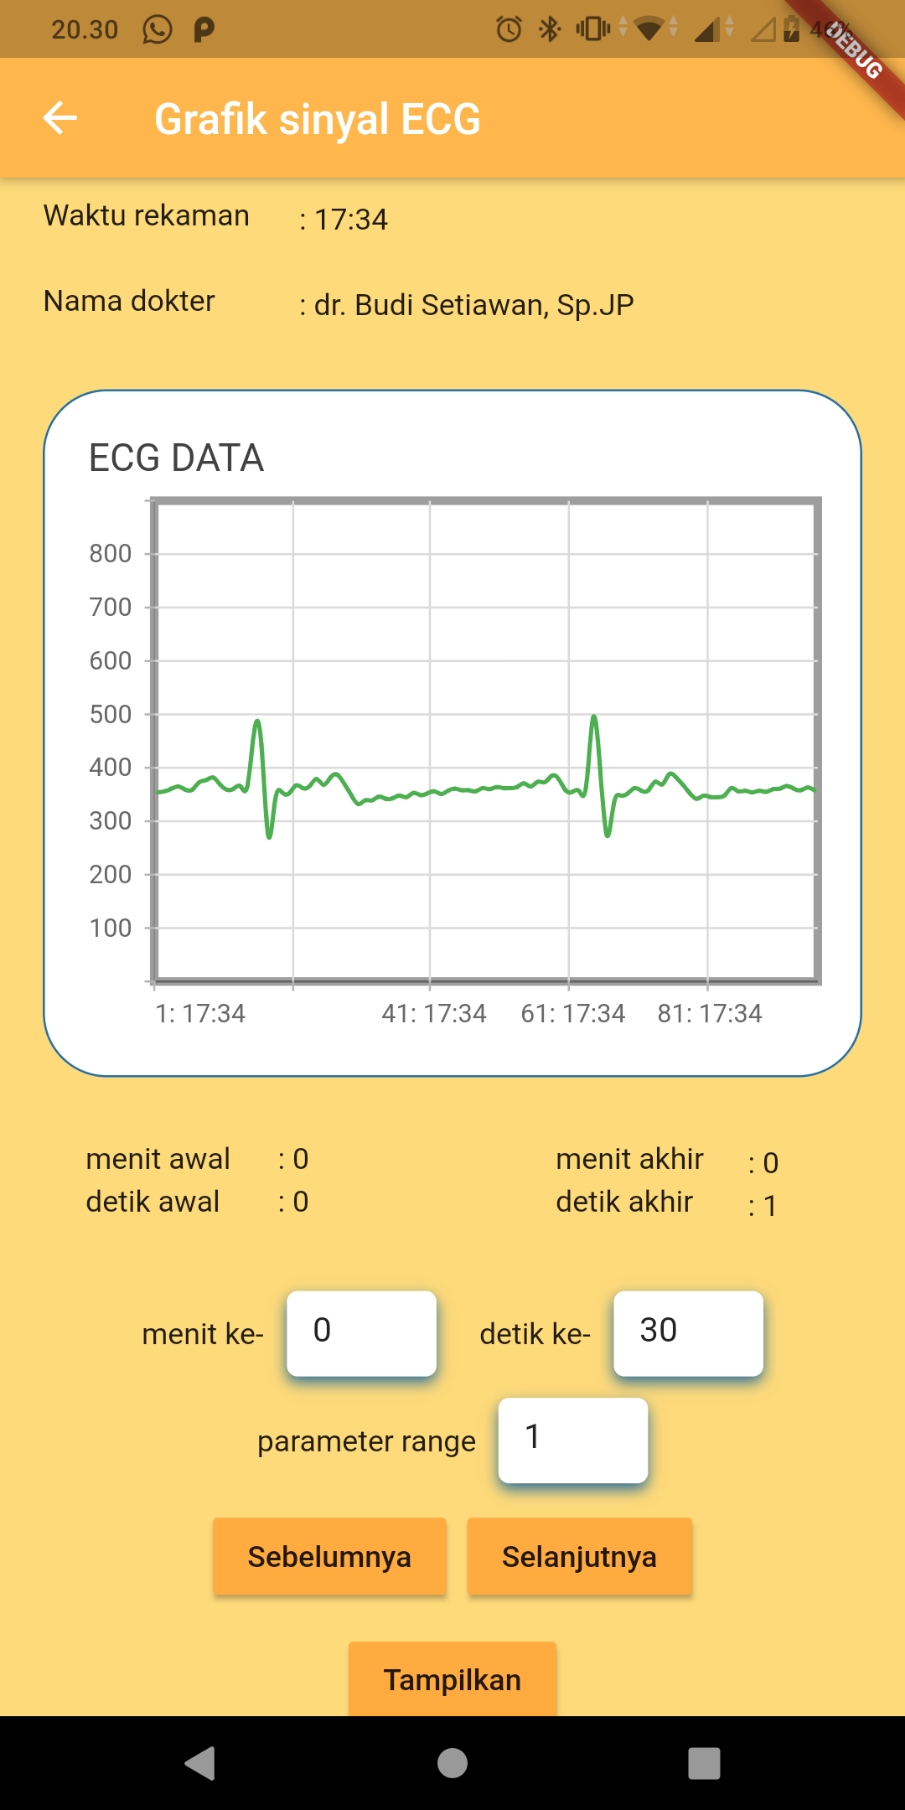
\includegraphics[width=0.45\textwidth]{img/grafikECGapps.jpg}
	\caption{Grafik ECG yang ditampilkan pada aplikasi.}
	\label{fig:4.0}
\end{figure}
Sedangkan grafik ECG yang ditampilkan pada serial ploter Arduino IDE ditunjukkan pada gambar berikut.
\begin{figure}[H] \centering
	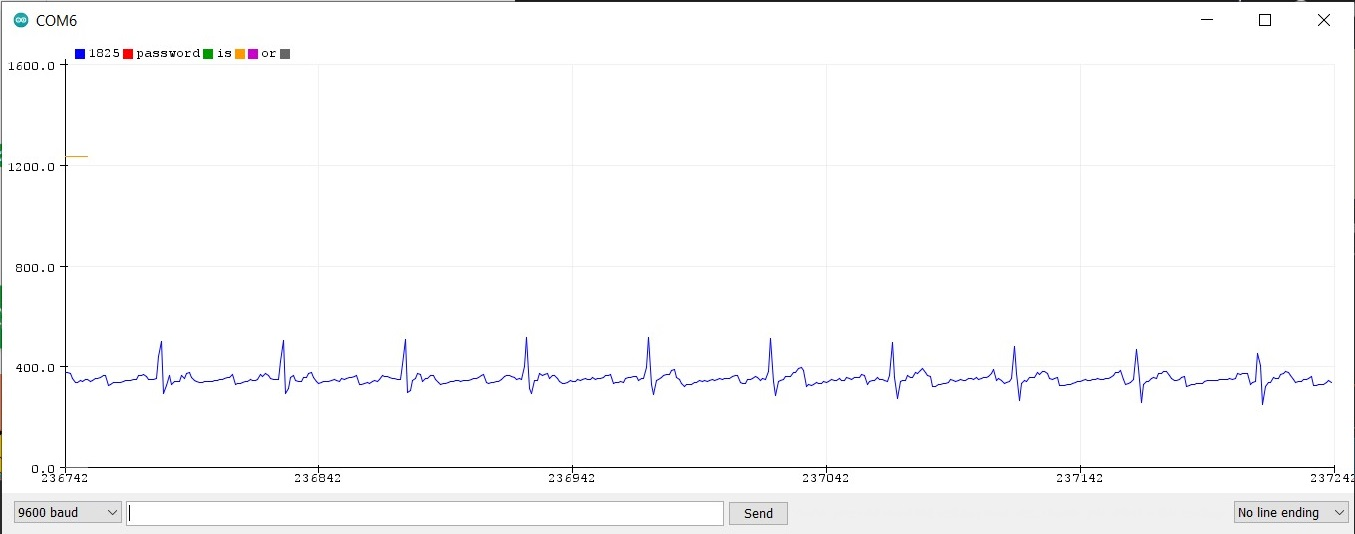
\includegraphics[width=1\textwidth]{img/ujisesuaidataIDE.jpg}
	\caption{Grafik ECG yang ditampilkan pada serial ploter Arduino IDE.}
	\label{fig:4.1}
\end{figure}

Berdasarkan kedua gambar diatas, apabila dibandingkan maka kedua gambar tersebut cukup mirip. Dengan demikian berarti hasil grafik ECG yang ditampilkan oleh aplikasi android cukup sesuai dengan grafik ECG yang ditampilkan oleh serial ploter Arduino IDE.
\vspace{1ex}

